\begin{figure}[H]
\centering
%
\begin{subfigure}{0.8\textwidth}
  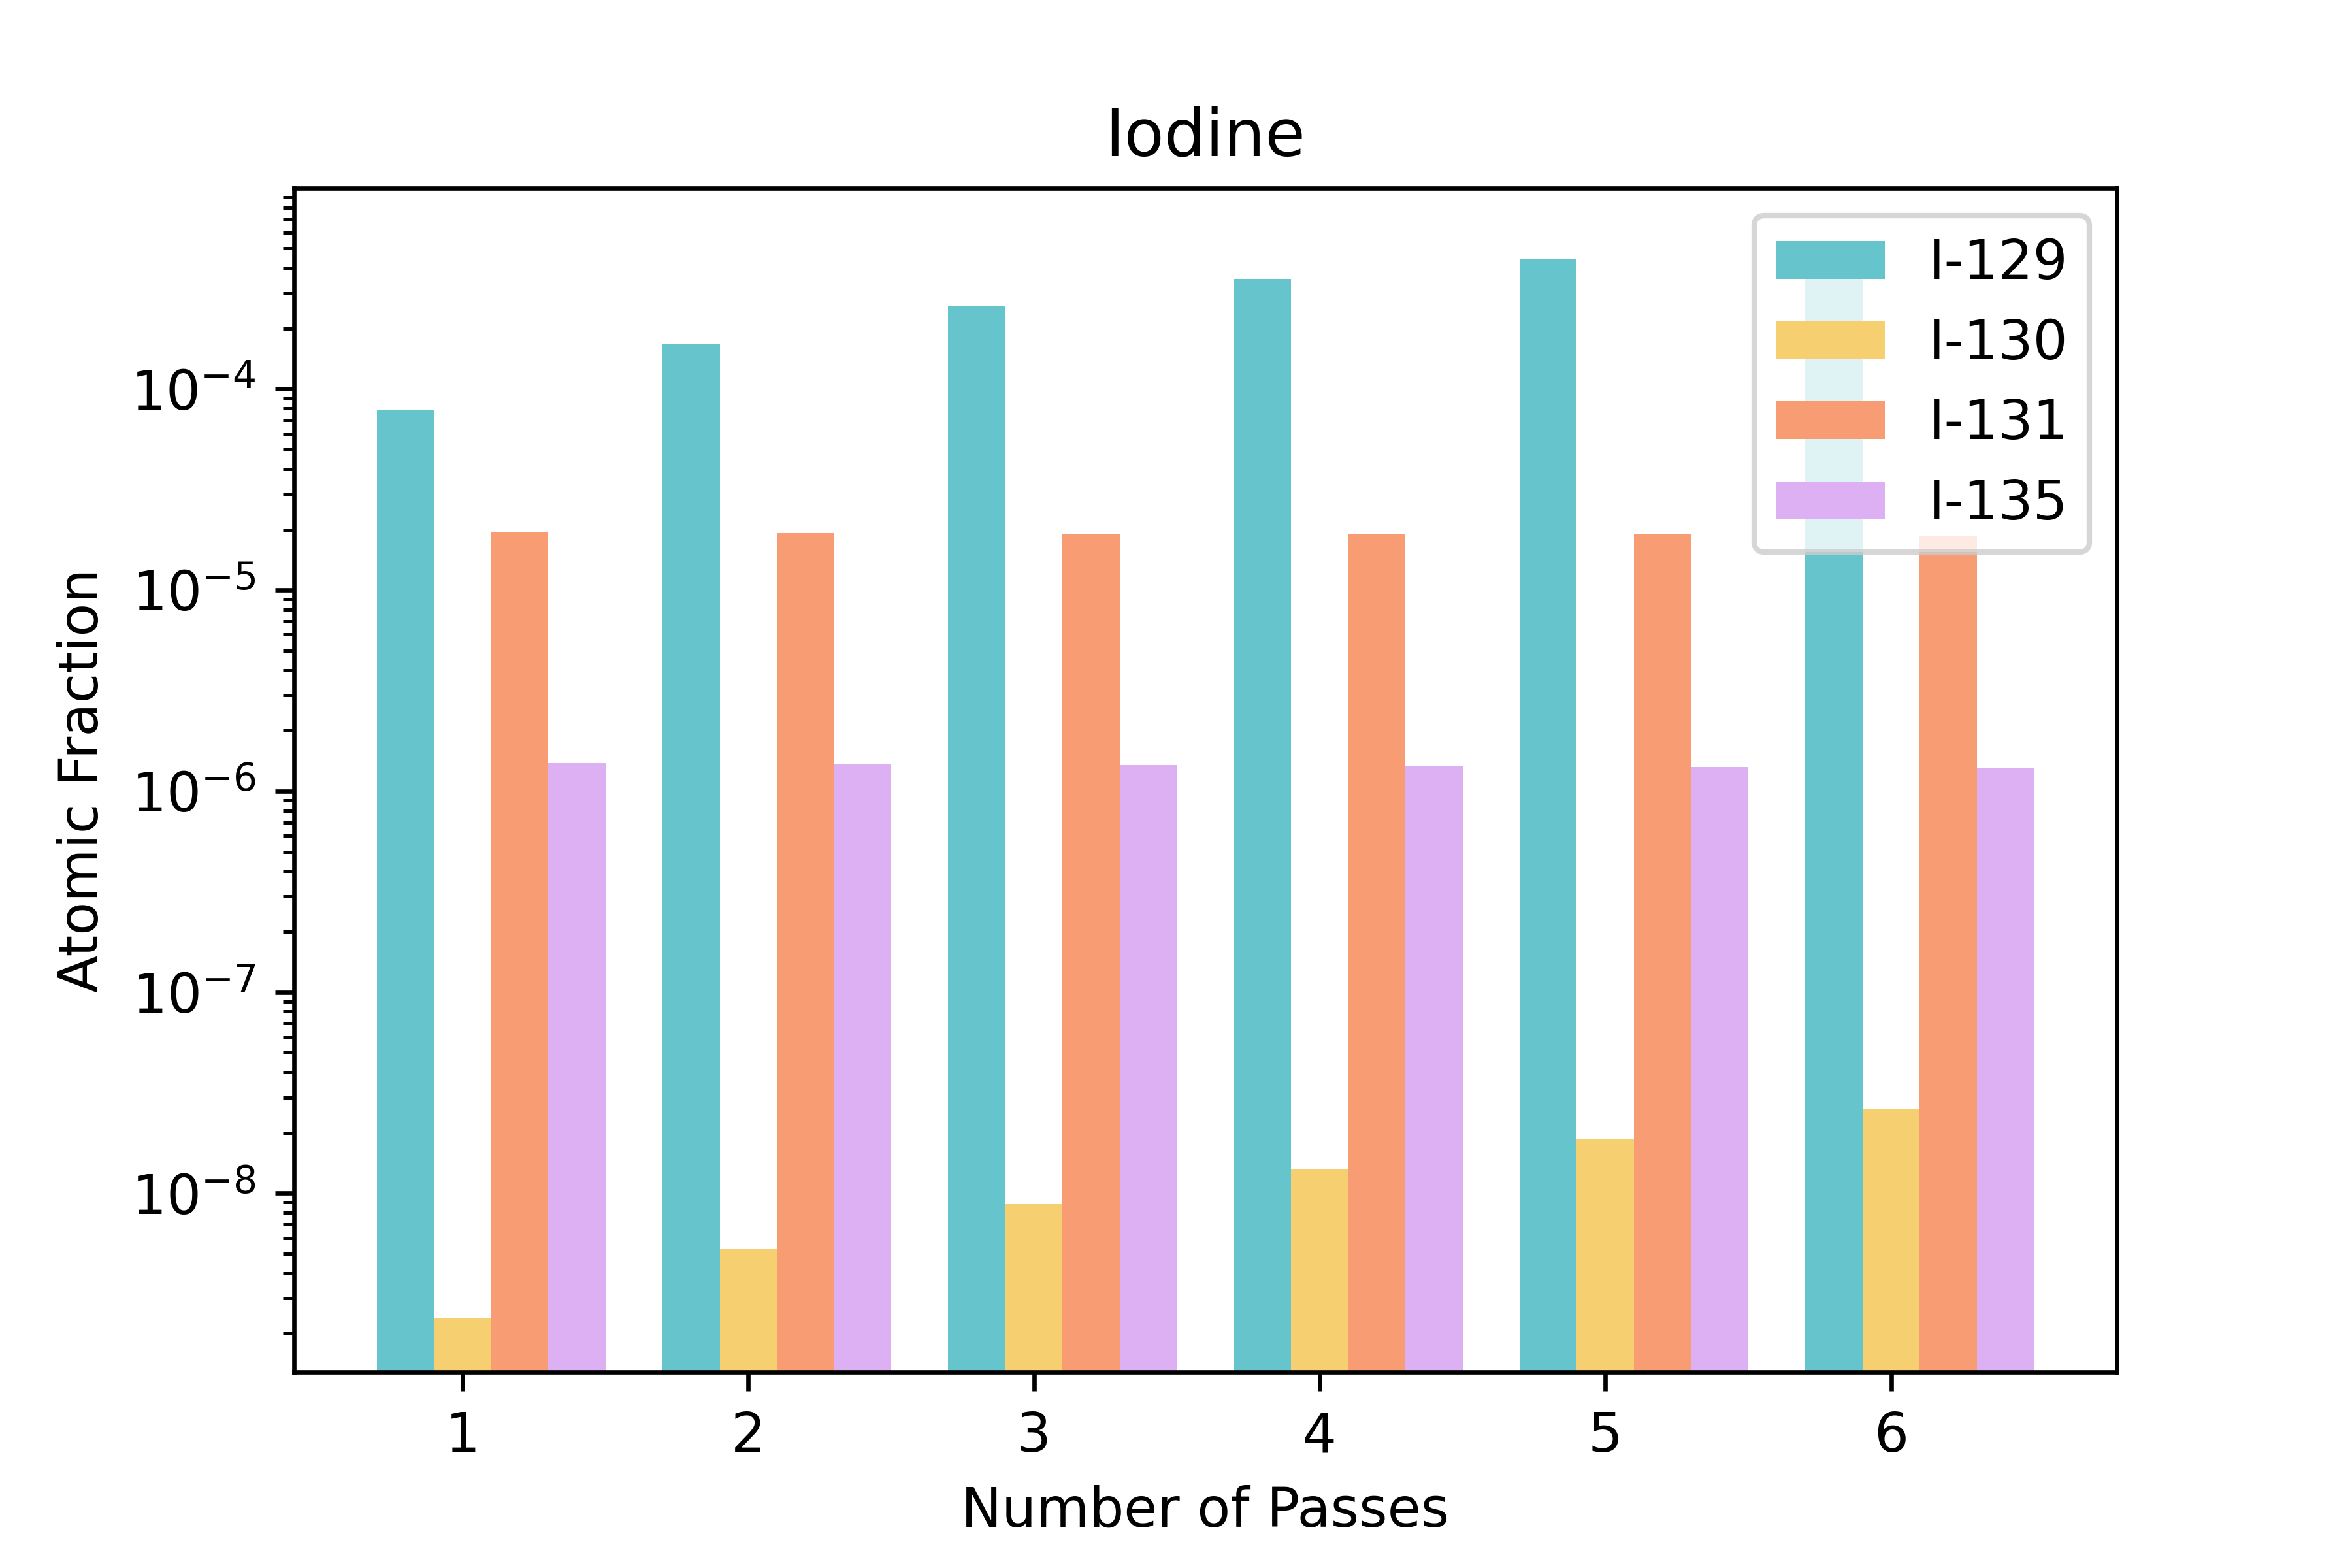
\includegraphics[width=\linewidth]{figures/compositions/iodine}
  \caption{Iodine isotope buildup over six burnup stages}
  \label{fig:i}
\end{subfigure}%

\begin{subfigure}{0.8\textwidth}
  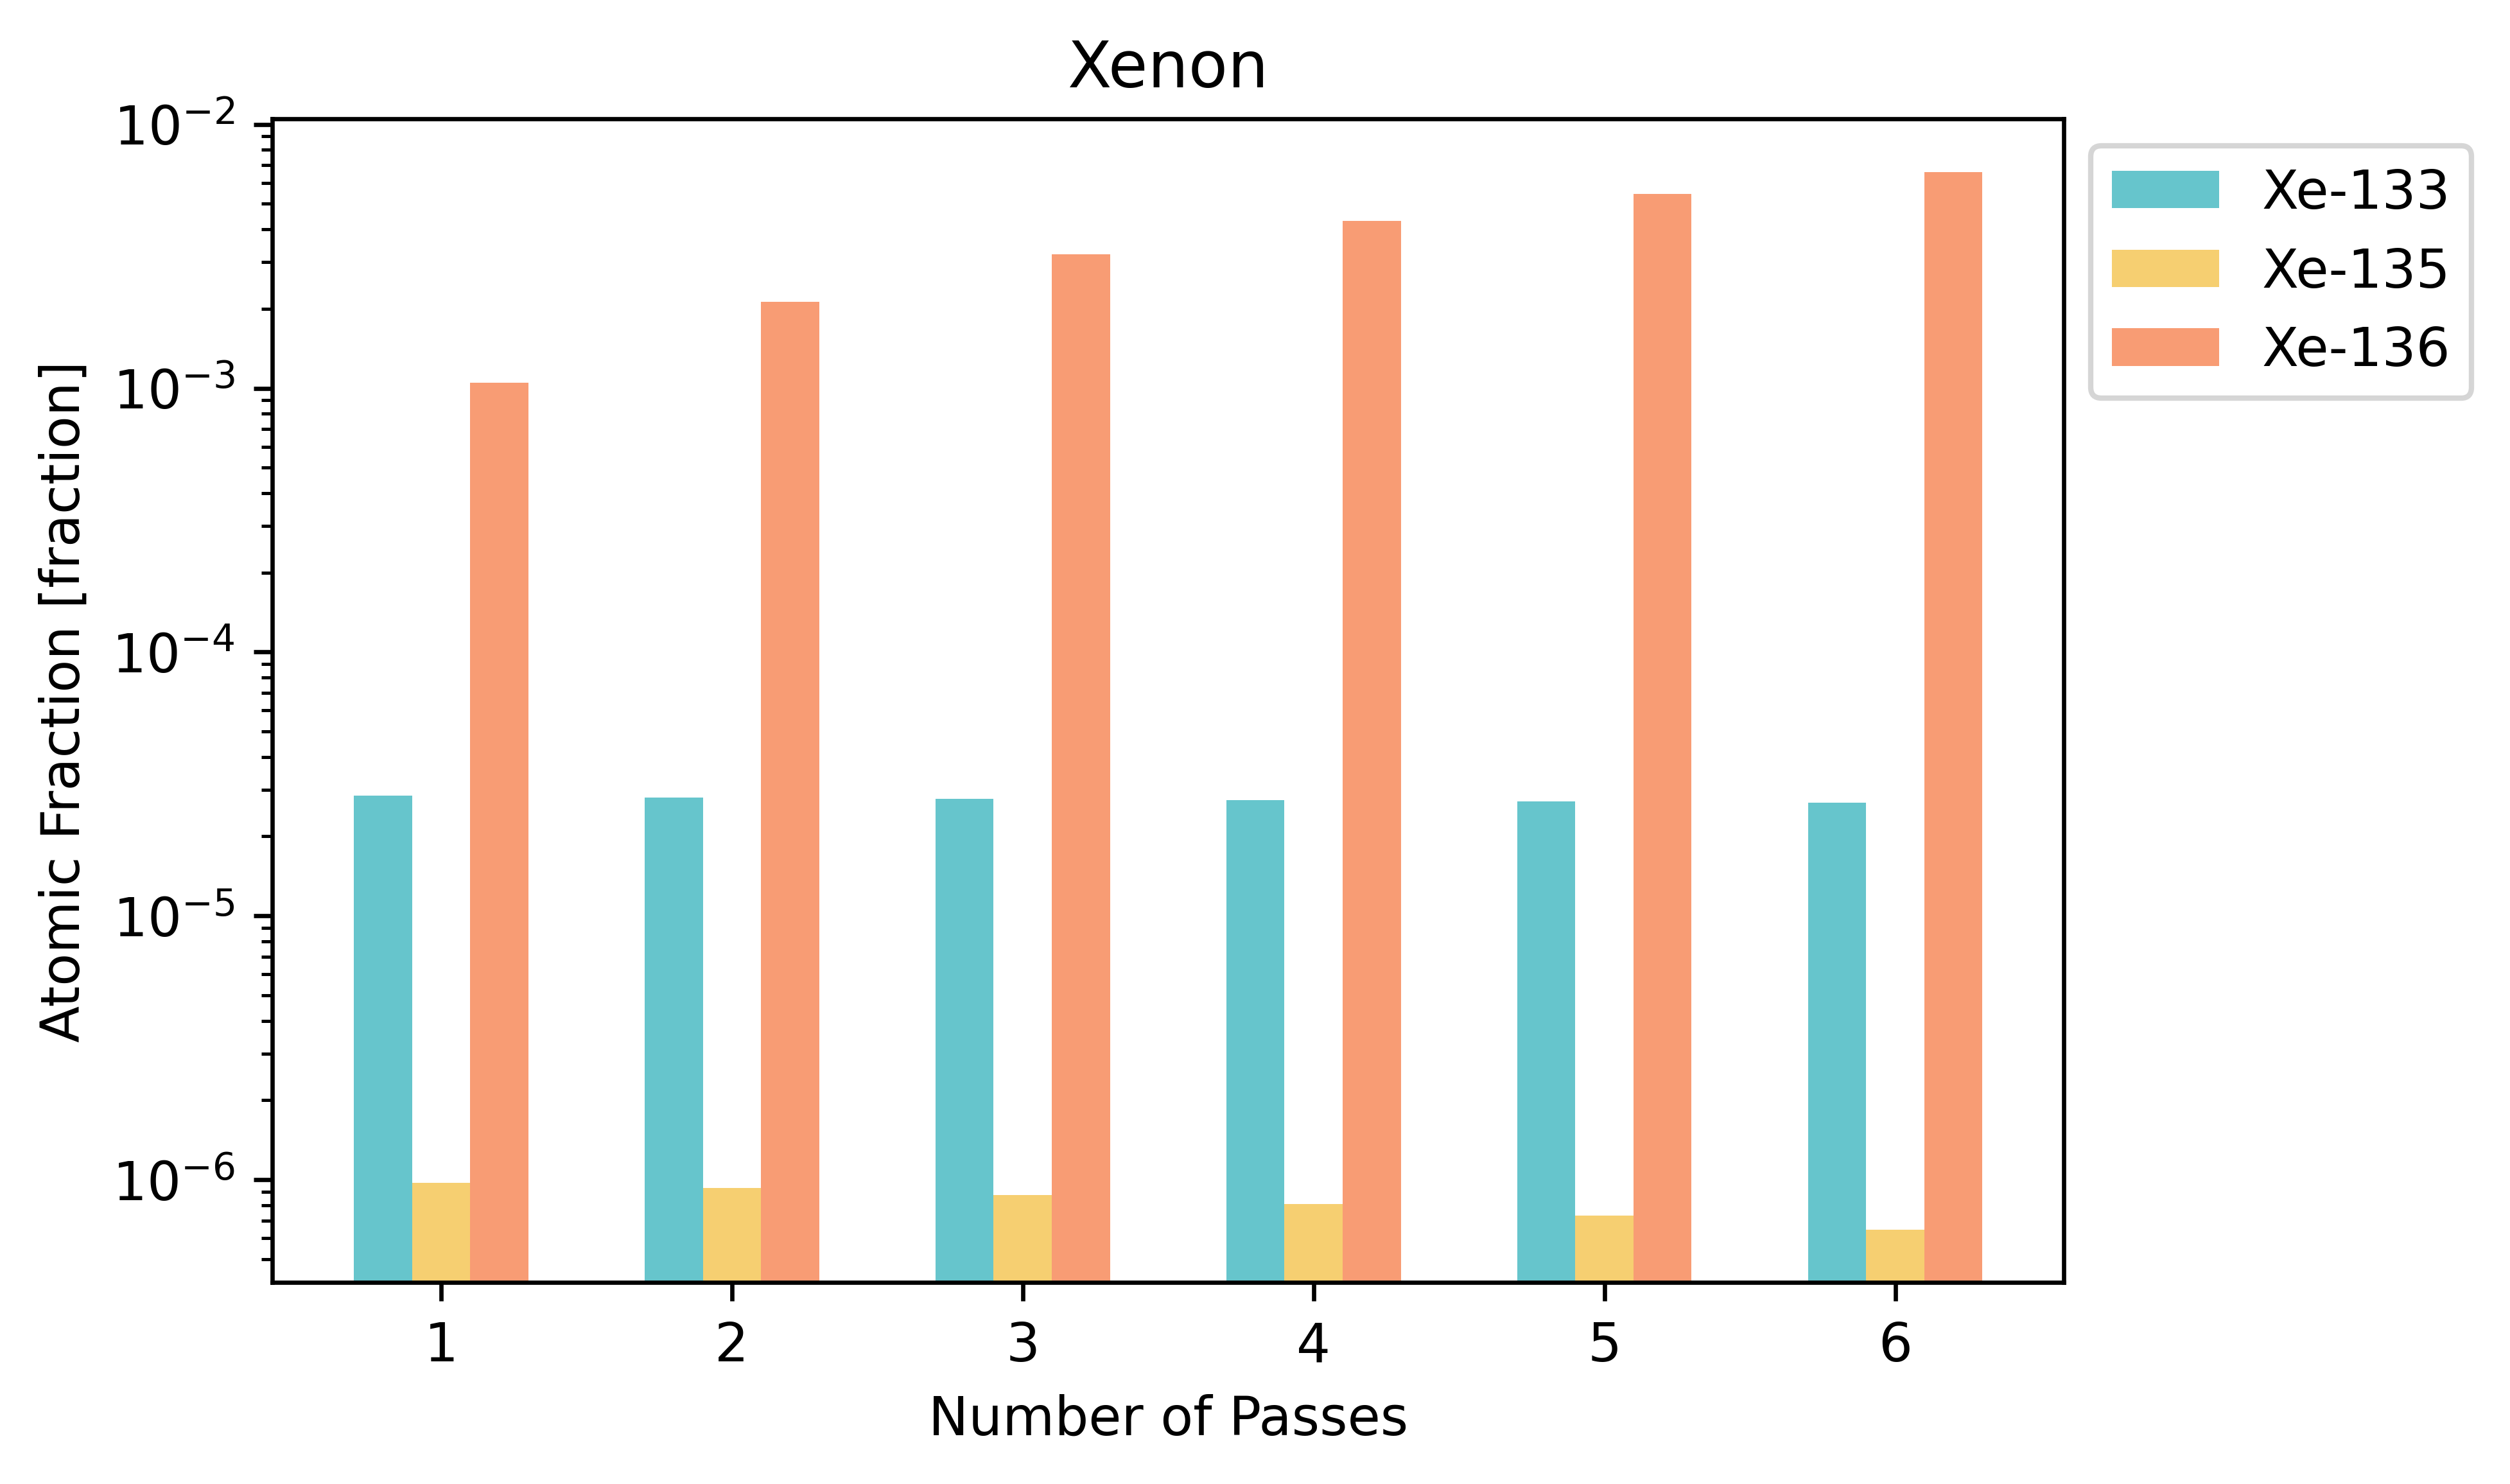
\includegraphics[width=\linewidth]{figures/compositions/xenon}
  \caption{Xenon isotope buildup over six burnup stages}
  \label{fig:xe}
\end{subfigure}%

\caption[Evolution of Safety Relevant Isotopic Concentrations in Pebbles of Sangamon20 over Six Six-Month Passes]{Evolution of Safety Relevant Isotopic Concentrations in Pebbles of Sangamon20 over Six Six-Month Passes (measured in atomic fraction)}
\end{figure}

\begin{figure}[H]\ContinuedFloat
\centering

\begin{subfigure}{0.8\textwidth}
  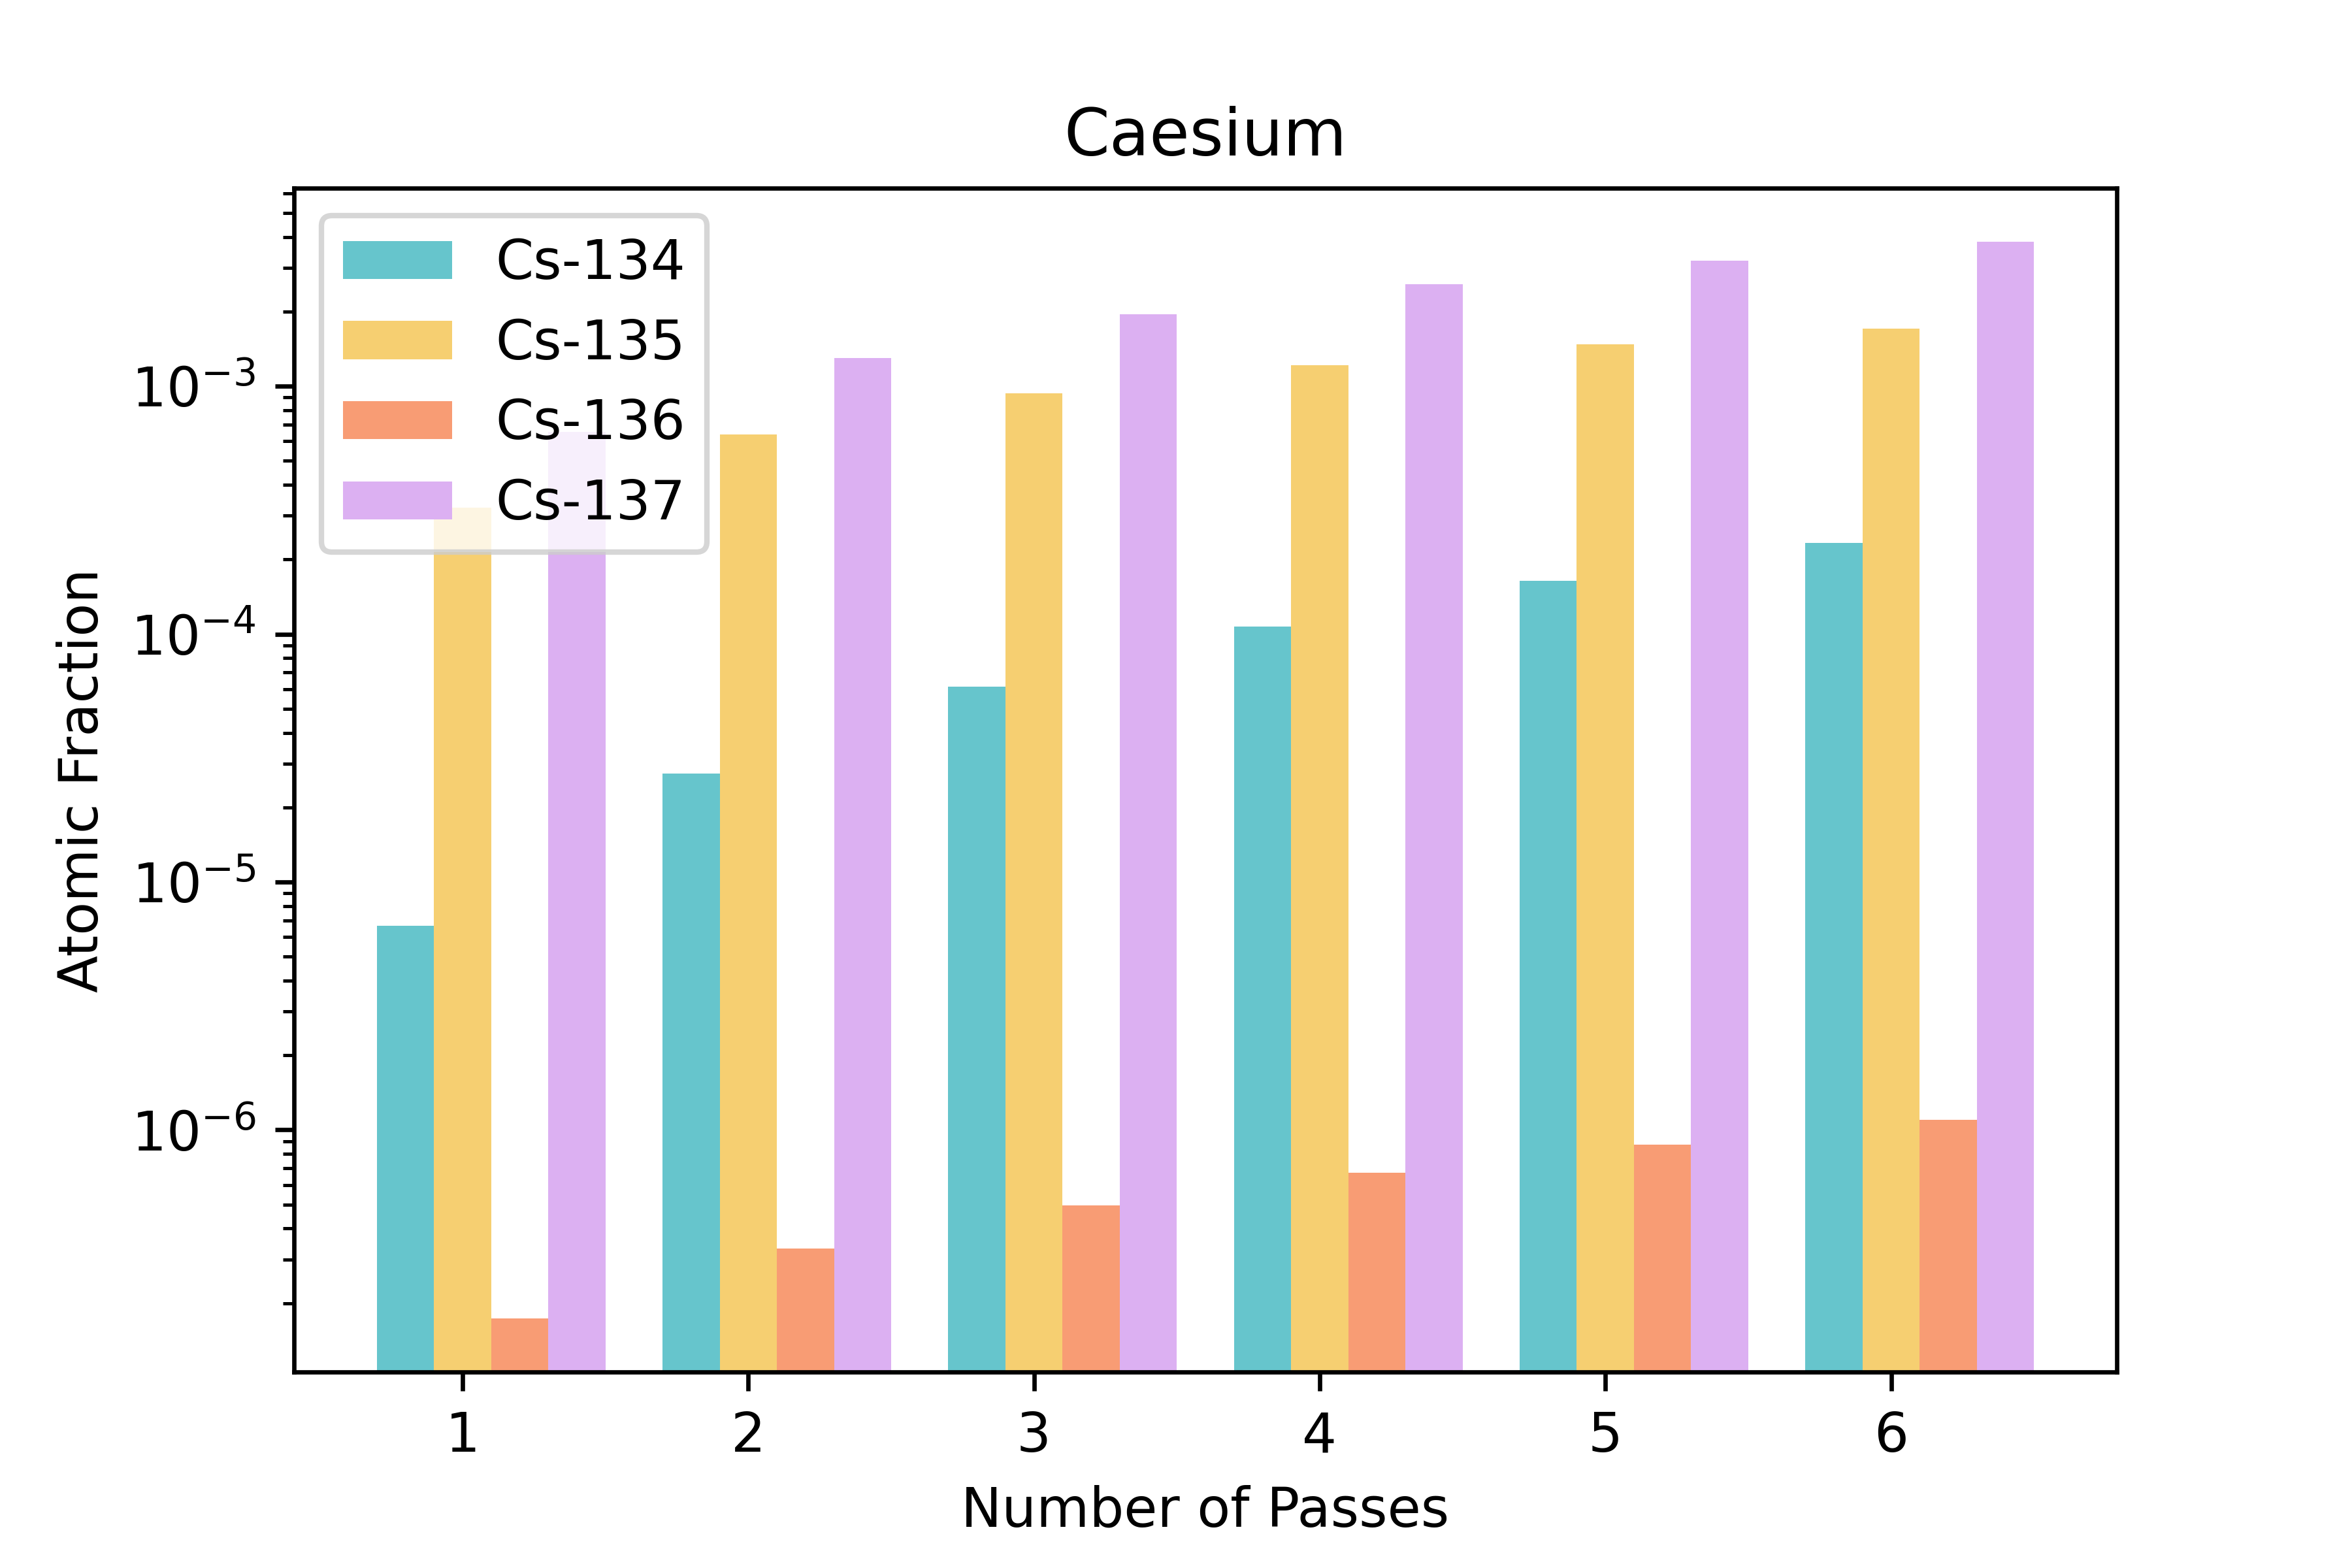
\includegraphics[width=\linewidth]{figures/compositions/caesium}
  \caption{Cesium isotope buildup over six burnup stages}
  \label{fig:cs}
\end{subfigure}%


\begin{subfigure}{0.8\textwidth}
  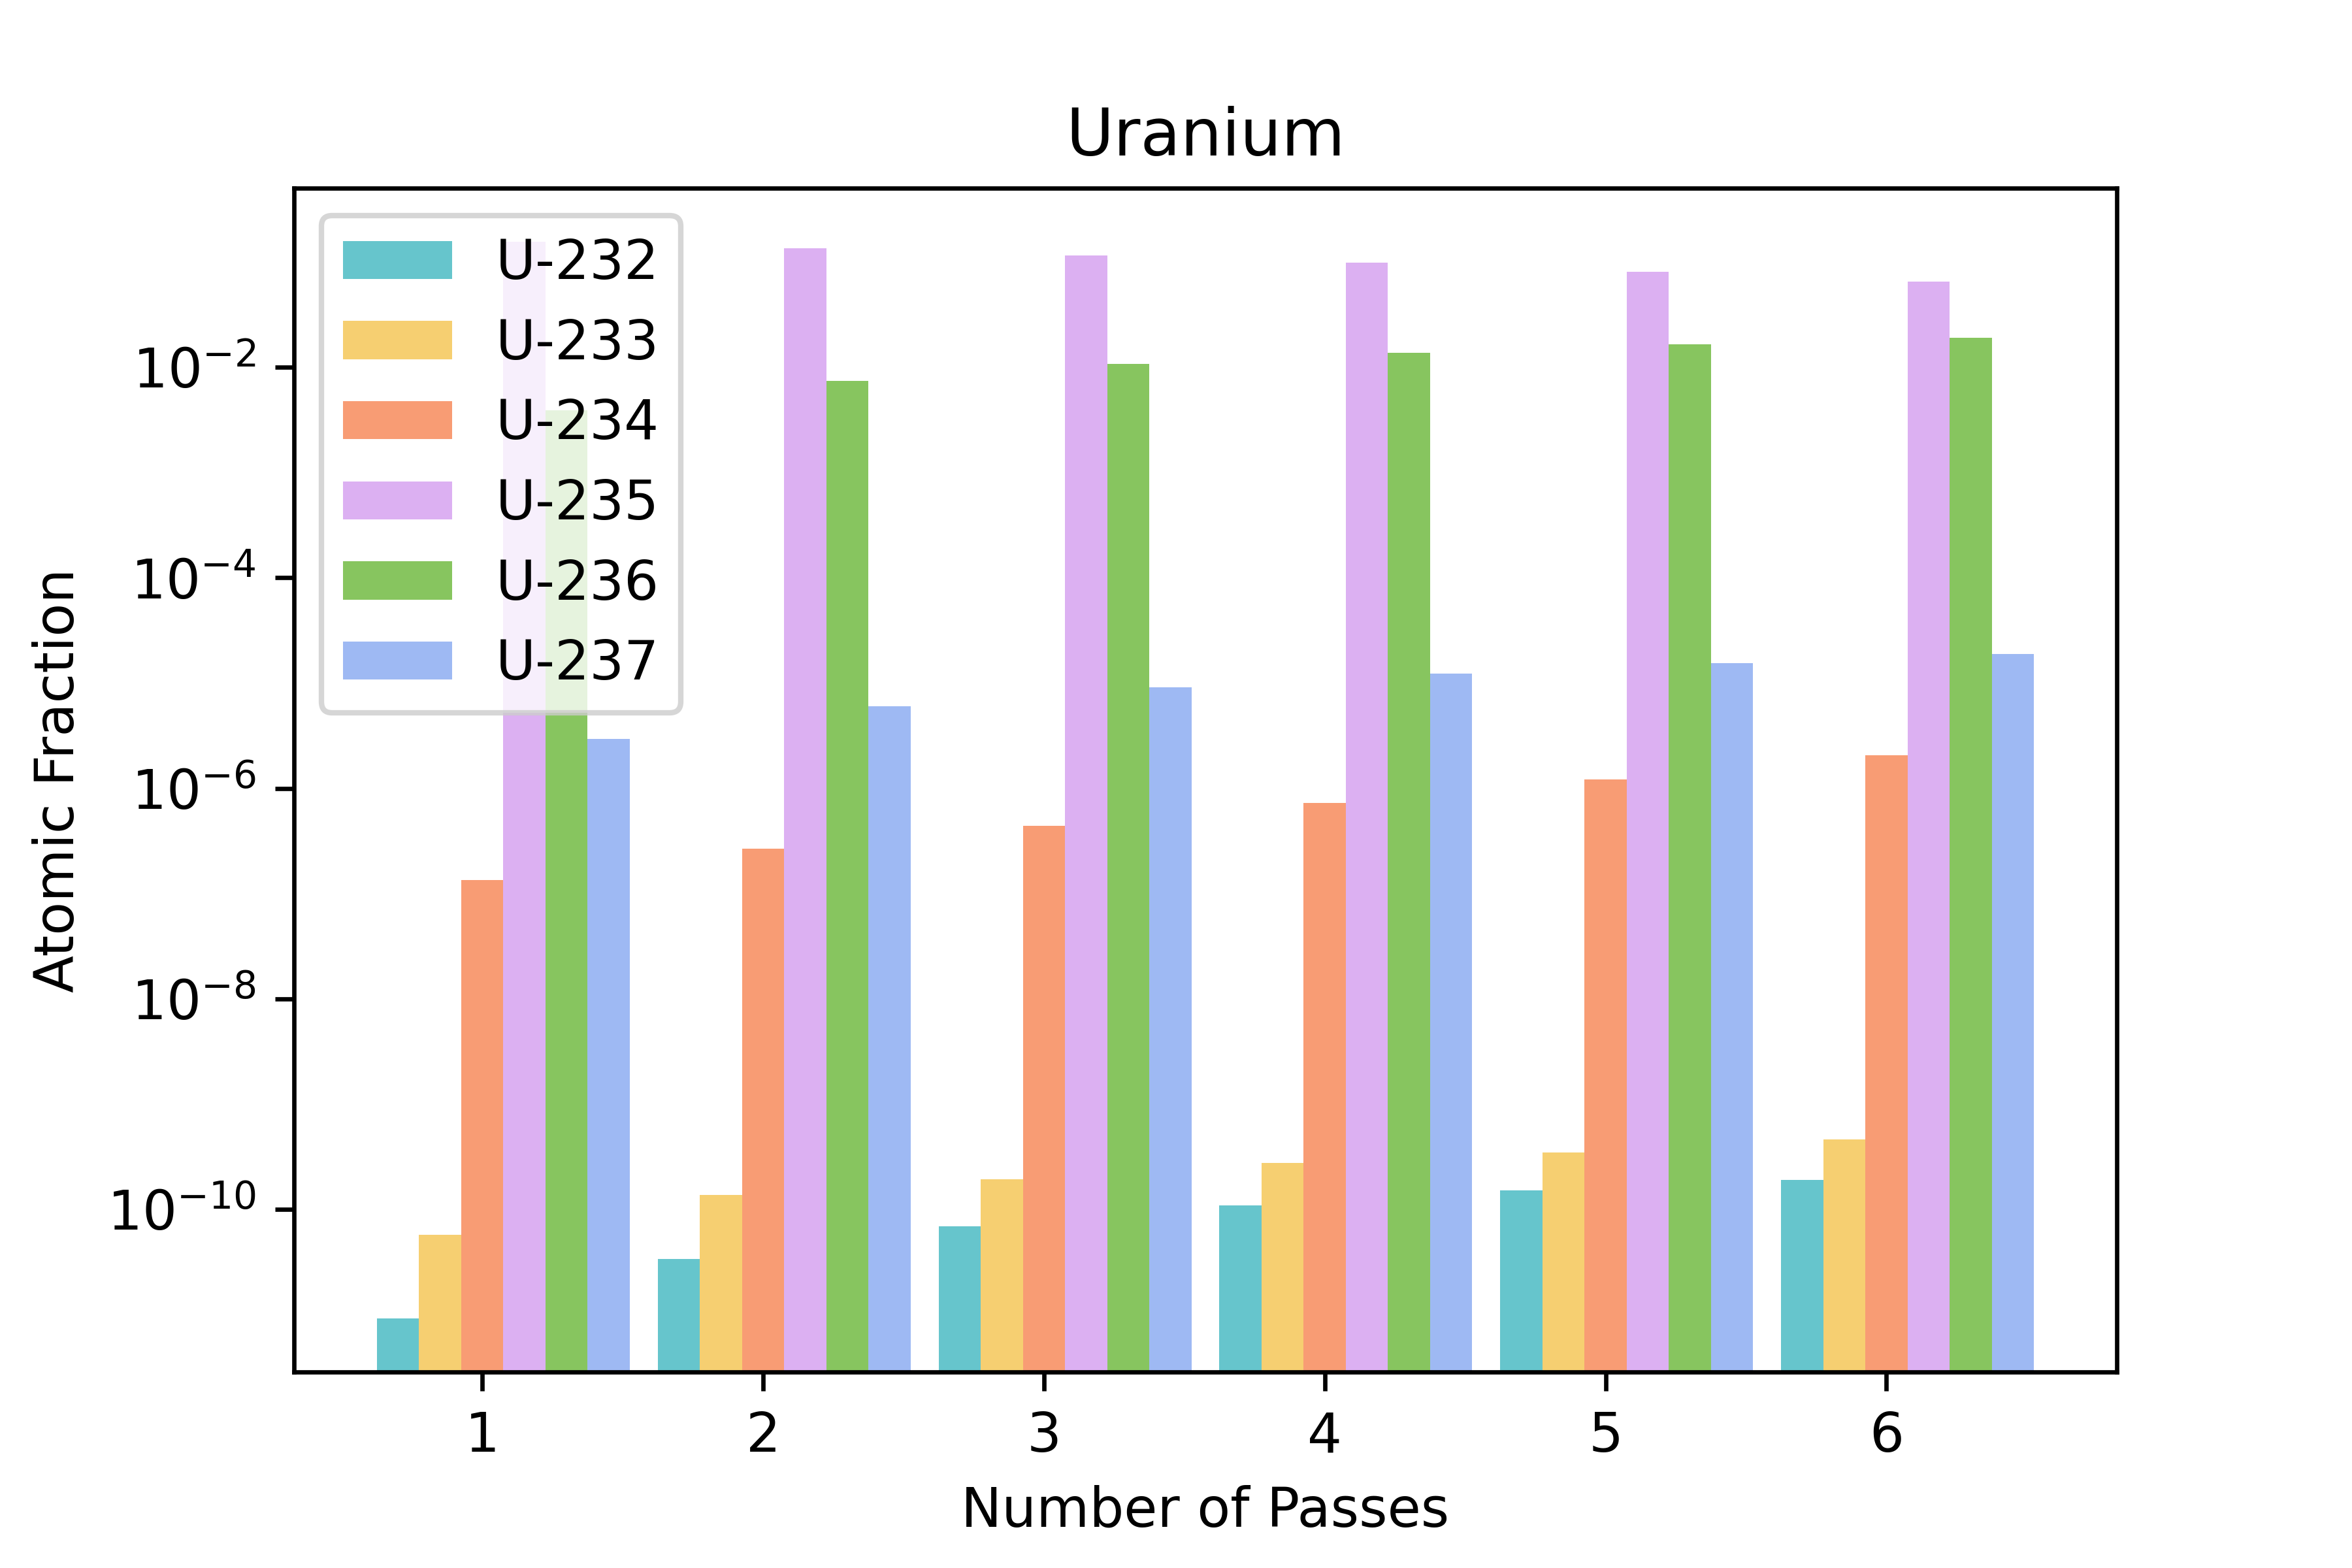
\includegraphics[width=\linewidth]{figures/compositions/uranium}
  \caption{Uranium isotope buildup over six burnup stages}
  \label{fig:u}
\end{subfigure}%

\caption[]{(cont.)}
\end{figure}

\begin{figure}[H]\ContinuedFloat
\centering

\begin{subfigure}{0.8\textwidth}
  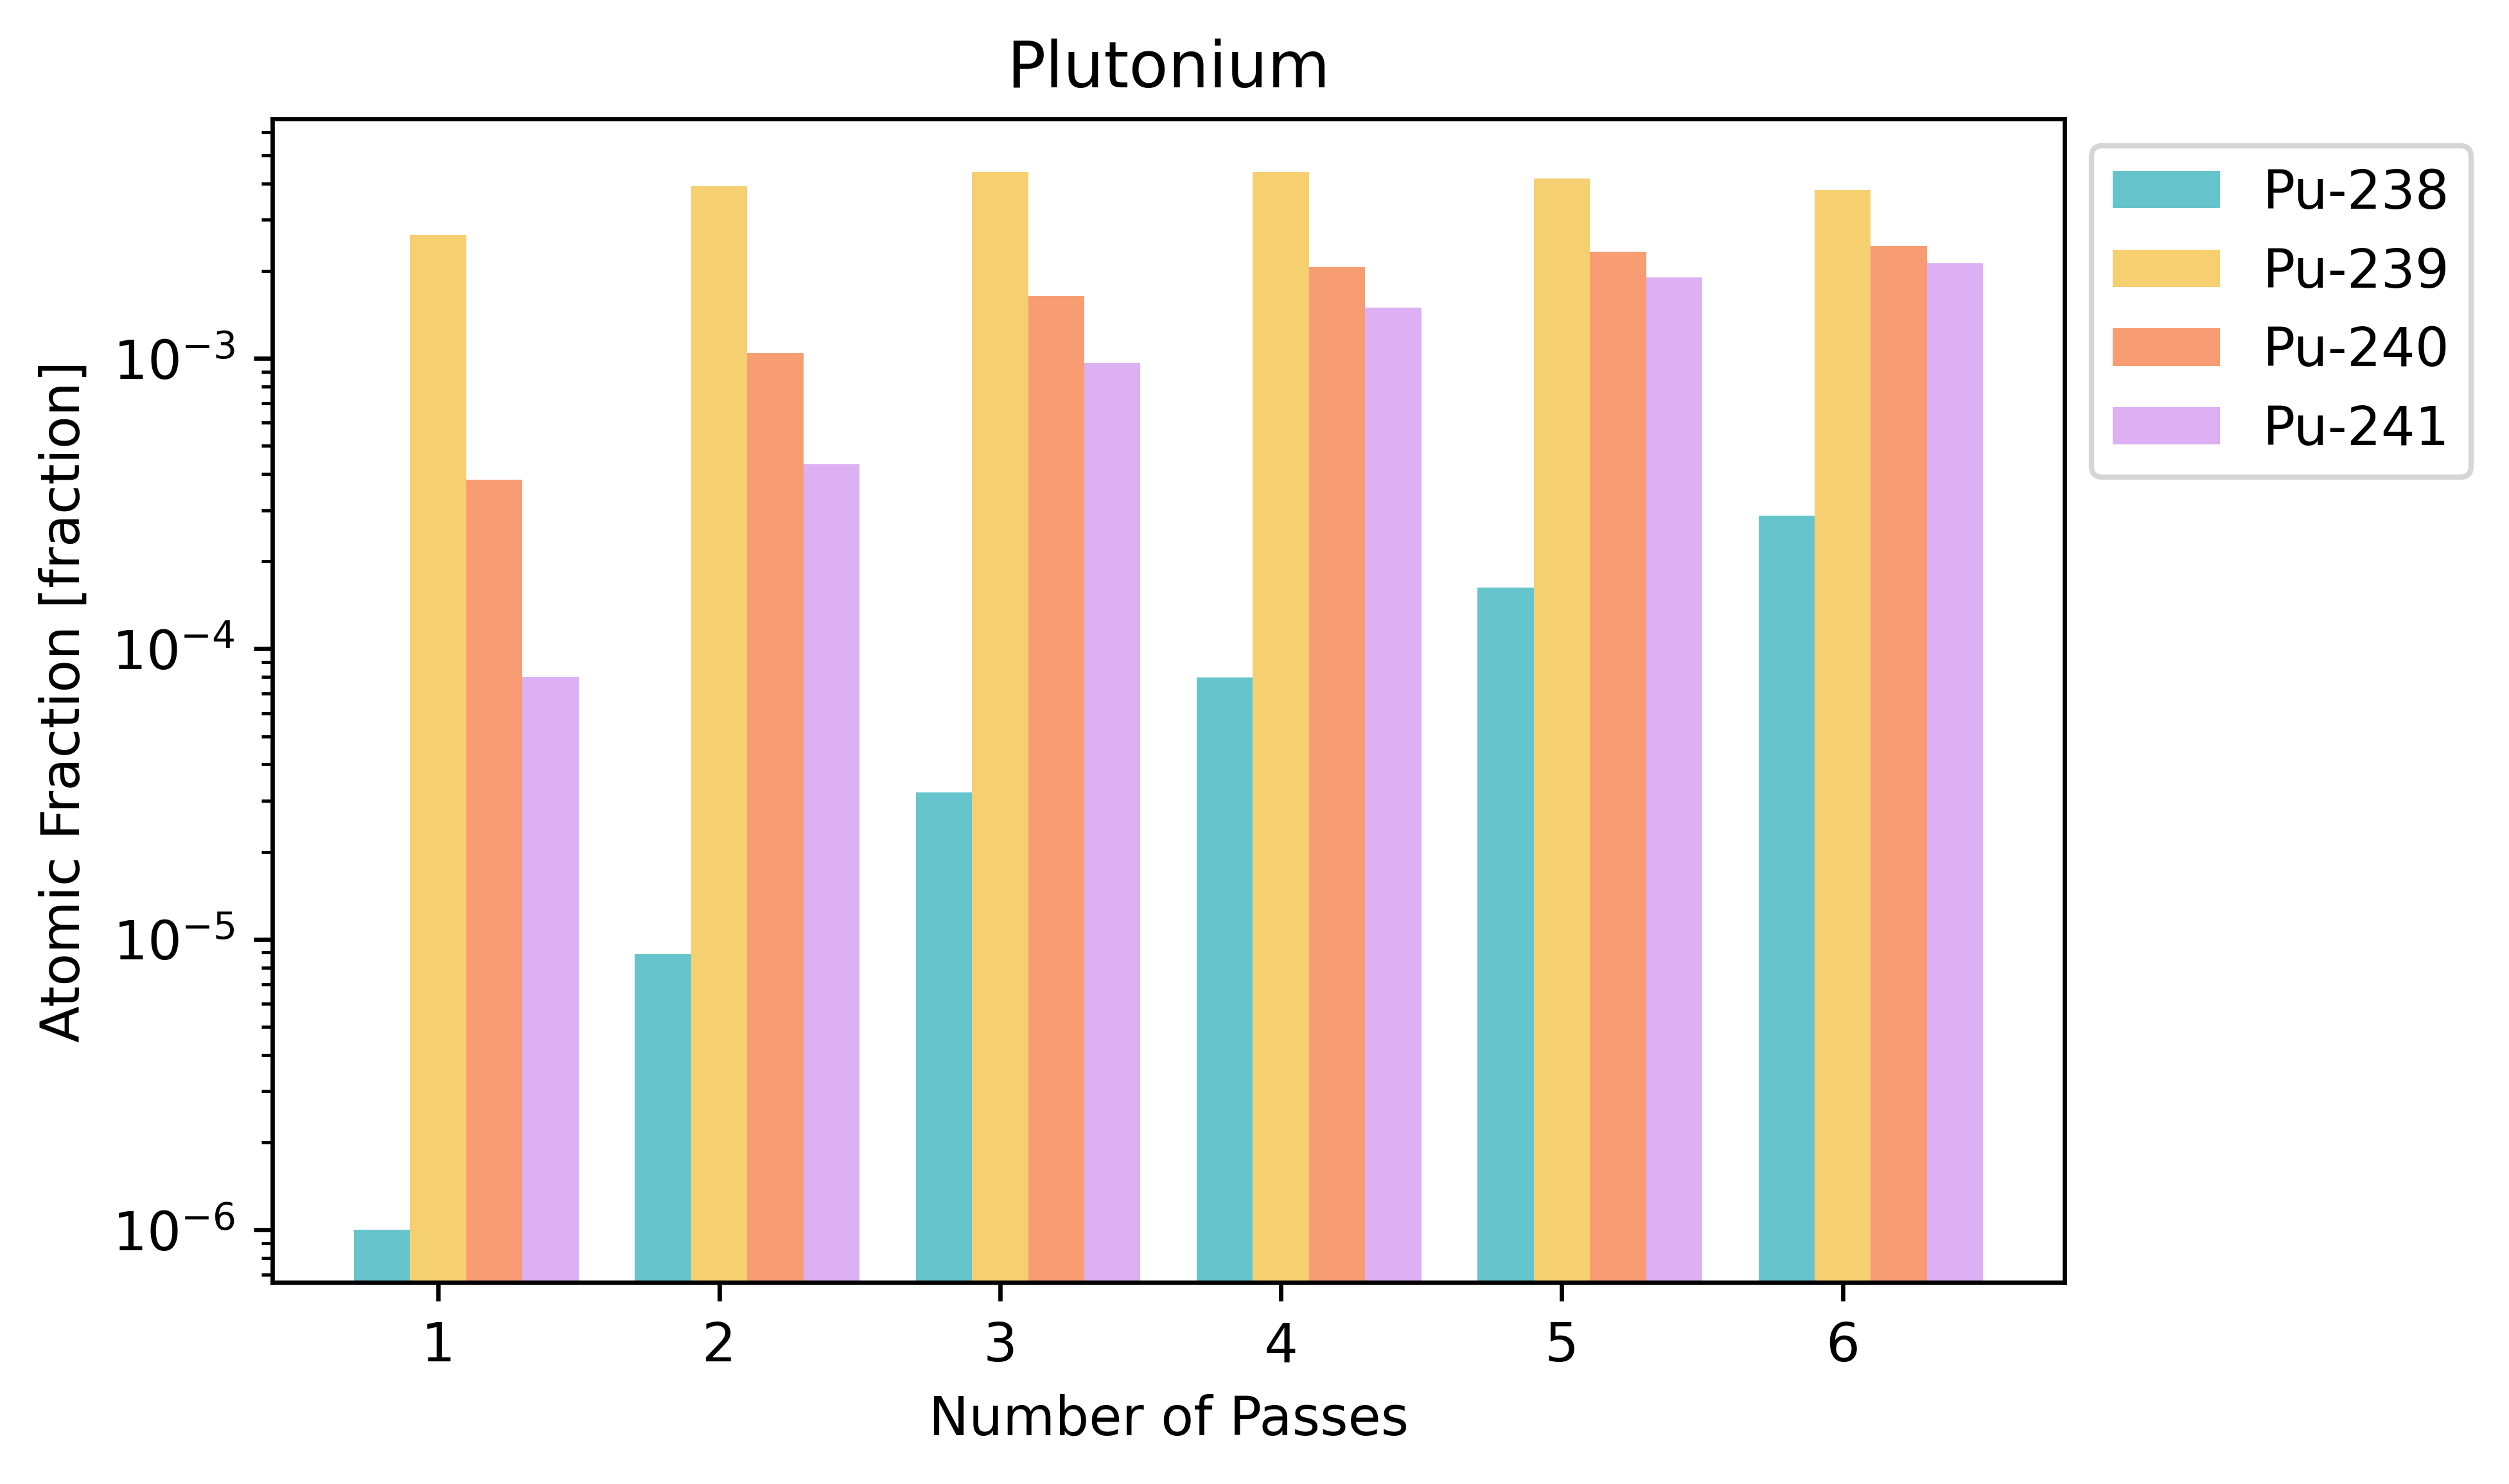
\includegraphics[width=\linewidth]{figures/compositions/plutonium}
  \caption{Plutonium isotope buildup over six burnup stages}
  \label{fig:pu}
\end{subfigure}%

\caption[]{(cont.)}
\label{fig:comps}
\end{figure}